% Created 2020-10-05 Mon 20:43
% Intended LaTeX compiler: pdflatex
\documentclass[11pt]{article}
\usepackage[utf8]{inputenc}
\usepackage[T1]{fontenc}
\usepackage{graphicx}
\usepackage{grffile}
\usepackage{longtable}
\usepackage{wrapfig}
\usepackage{rotating}
\usepackage[normalem]{ulem}
\usepackage{amsmath}
\usepackage{textcomp}
\usepackage{amssymb}
\usepackage{capt-of}
\usepackage{hyperref}
\author{Heitor Lourenço Werneck \\github.com/heitor57\\{\href{mailto:heitorwerneck@hotmail.com}{heitorwerneck@hotmail.com}}}
\usepackage[portuguese]{babel}
\usepackage{mathtools}
\usepackage[binary-units=true]{siunitx}
\usepackage[top=0.5cm,bottom=1.5cm,left=2cm,right=2cm]{geometry}
\usepackage{mdframed}
\usepackage{listings}
\usepackage{algpseudocode}
\usepackage[Algoritmo]{algorithm}
\usepackage{tikz}
\usepackage{xcolor}
\usepackage{colortbl}
\usepackage{graphicx,wrapfig,lipsum}
\usepackage{pifont}
\usepackage{subfigure}
\usepackage{rotating}
\usepackage{multirow}
\usepackage{tablefootnote}
\usepackage{enumitem}
\usepackage{natbib}
\usepackage{dblfloatfix}
\usepackage{color, colortbl}
\usepackage{chngcntr}
\usepackage{epstopdf}
\date{\today}
\title{Algoritmo genético\\\medskip
\large Algoritmos Bioinspirados}
\hypersetup{
 pdfauthor={Heitor Lourenço Werneck},
 pdftitle={Algoritmo genético},
 pdfkeywords={},
 pdfsubject={},
 pdfcreator={Emacs 27.1 (Org mode 9.3)}, 
 pdflang={Portuguese}}
\begin{document}

\maketitle
\usetikzlibrary{arrows, fit, matrix, positioning, shapes, backgrounds,intersections}
\usetikzlibrary{decorations.pathreplacing}
\usetikzlibrary{automata, positioning, arrows}
\usetikzlibrary{calc}

\definecolor{bg}{rgb}{0.95,0.95,0.95}
\BeforeBeginEnvironment{minted}{\begin{mdframed}[backgroundcolor=bg]}
\AfterEndEnvironment{minted}{\end{mdframed}}
\numberwithin{equation}{section}
\algnewcommand{\IfThenElse}[3]{% \IfThenElse{<if>}{<then>}{<else>}
  \State \algorithmicif\ #1\ \algorithmicthen\ #2\ \algorithmicelse\ #3}

% Define block styles
\tikzstyle{decision} = [diamond, draw, fill=blue!20, 
    text width=4.5em, text badly centered, node distance=3cm, inner sep=0pt]
\tikzstyle{block} = [rectangle, draw, fill=blue!20, 
    text width=5em, text centered, rounded corners, minimum height=4em]
\tikzstyle{line} = [draw, -latex']
\tikzstyle{cloud} = [ellipse, draw, fill=red!20, 
    text width=5em, text centered, rounded corners, minimum height=2em]
%\tikzstyle{cloud} = [draw, ellipse,fill=red!20, node distance=3.5cm,
%    minimum height=2em]


\lstset{
  basicstyle=\ttfamily,
  columns=fullflexible,
  frame=single,
  breaklines=true,
  postbreak=\mbox{\textcolor{red}{$\hookrightarrow$}\space},
}
\DeclarePairedDelimiter\ceil{\lceil}{\rceil}
\DeclarePairedDelimiter\floor{\lfloor}{\rfloor}

% Numbering fix
\counterwithout{equation}{section} % undo numbering system provided by phstyle.cls
%\counterwithin{equation}{chapter}  % implement desired numbering system


\section{Introdução}
\label{sec:orgb303907}
Algoritmos genéticos se referem a uma família de modelos computacionais inspirados na evolução(seleção natural e genética). Esses algoritmos representam a solução problema atráves de estruturas semelhantes a cromossomos e aplicam operadores de recombinação para preservar os dados/informações vitais \cite{whitley94_genet_algor_tutor,goldenberg1989genetic}. Normalmente um algoritmo genético será baseado em população e usará operadores de seleção e recombinação para buscar uma solução no espaço de busca \cite{whitley94_genet_algor_tutor}.

Algoritmos genéticos são utilizados em diversos cenários pela natureza generalista de seu modelo, como por exemplo: sistemas de recomendação \cite{naruchitparames2011friend,silva2010graph}; visão computacional \cite{gong2004quadtree}; robôs de limpeza \cite{yakoubi2016path}; recuperação de informação \cite{vrajitoru1998crossover} e agendamento de voos \cite{lee2007multi}.

Os algoritmos genéticos também possuem a capacidade de fazer \emph{exploitation} e \emph{exploration} que são características de modelos estado da arte em diversas áreas, como por exemplo: \emph{Multi-Armed Bandits}; Nuvem de partículas e outros. Uma característica extremamente importante para diversos cenários.

Esse trabalho consiste na implementação e análise de um algoritmo genético para solução de um problema de otimização de uma função.

\section{Problema}
\label{sec:orgf659f66}

O problema é simples e consiste na minimização da função da equação \ref{eq:fo}. 
\begin{equation}
\label{eq:fo}
F_o(x) = -20\epsilon^{-0.2}\sqrt{\frac{1}{n}\sum x_i^2} - \epsilon^{\frac{1}{n}\sum cos(2\pi x_i)} + 20 + \epsilon
\end{equation}

É importante notar que como o problema será representado em um sistema computacional como um vetor de números binários então o espaço de busca terá \(2^{\text{bits}}\) possibilidades de solução. Isso mostra que é um problema difícil, pois possui uma complexidade de ordem exponencial no espaço de soluções, por isso é importante usar alguma heurística ou meta-heurística (que no caso é algoritmo genético) para solucionar esse problema caso não tenha solução analítica viável.

\section{Solução}
\label{sec:orgccd068f}

A estruturas basicas para o algoritmo foram determinadas da seguinte forma: os genes são números binários de tamanho \(\# Bits\) (definido posteriormente) tal que é transformado em decimal dentro de um espaço linear \([x_{min},x_{max}]\) para ser avaliado pela função objetivo. A estrutura foi feita dessa forma pois permite mais flexibilidade nas operações genéticas e também delimita um espaço de busca discreto que pode ajudar na solução de alguns problemas. 

O intervalo de busca de valores foi dentro do domínio \(x_{min} = -2\) e \(x_{max} = 2\), isso por que foi analisado que dentro dessa espaço há bons valores para minimização da função. Foi utilizado uma população com tamanho 50 e o número de iterações utilizados foi de 20. O espaço linear delimitado dentro deste domínio contém \(2^{\# Bits}\) valores sendo \(\# Bits=6\) e 2 genes (\(\# Genes = 2\); genes de \(\# Bits\) bits) utilizados. Esses valores serão variados posteriormente para análise do comportamento do algoritmo.

A estrategia de seleção utilizada foi a roleta, tal que é selecionado dois indivíduos aleatórios na população e o indivíduo com maior aptidão (menor valor na função objetivo) será selecionado como o primeiro pai a compor o par de pais com probabilidade de 90\%. Após isso o processo é repetido excluindo o indivíduo já selecionado e dois pais são obtidos.

Para a intensificação do espaço de busca foi utilizado o cruzamento, tal que o algoritmo irá selecionar um ponto dentro do intervalo \([1,\# Bits \cdot \# Genes -2]\) e esse ponto irá ser utilizado para o particionamento dos pedaços do genoma para criação dos filhos. A taxa de cruzamento utilizada por padrão foi de 100\%.

Após isso é utilizado uma mutação na população, para diversificação da população, essa mutação é feita com base em uma probabilidade de cada celula ser alterada, no caso o valor padrão utilizado foi de 1\%.

Com a mutação nos filhos o processo de elitismo é feito na população anterior, uma porcentagem de indivíduos com maior aptidao é dado como entrada e esses indivíduos vão substituir os piores indivíduos da geração atual. Foi feito a abordagem por porcentagem ao invés de somente um indíviduo para ser possível a análise da variação do parâmetro. O valor padrão foi de 5\%.

Foi escolhido não mutar o indivíduos da elite para gerar uma curva de convergência sem oscilação.

\begin{table}[htbp]
\caption{Valores padrões para os parâmetros}
\centering
\begin{tabular}{lrl}
Parâmetro & Valor & Descrição\\
\(x_{min}\) & -2 & Limite inferior do espaço discreto de busca\\
\(x_{max}\) & 2 & Limite superior do espaço discreto de busca\\
\#População & 50 & Quantidade de indivíduos\\
\#Gerações & 50 & Quantidade de gerações\\
\#Bits & 6 & Tamanho do gene em bits\\
\#Genes & 2 & Quantidade de genes\\
Taxa de cruzamento & 1.0 & Taxa do número de indivíduos que vão cruzar\\
Taxa de elitismo & 0.05 & Taxa do número de indivíduos a serem preservados\\
Taxa de mutados & 1.0 & Taxa do número de indivíduos aptos a serem mutados da população total\\
Taxa de mutação & 0.01 & Probabilidade da mutação de um bit em um gene\\
Probabilidade do vencedor & 0.9 & Probabilidade do vencedor de uma disputa ser pai\\
\end{tabular}
\end{table}


Uma visão geral de como o algoritmo funciona é dado a seguir:
\begin{algorithm}
  \caption{Algoritmo genético}
  \begin{algorithmic}[1]
  \State Inicia a população com cromossomos aleatórios
  \For{$i=1$ to \#Gerações}
  \State Cruza os indivíduos utilizando torneio para selecionar os pais e de acordo com a taxa de cruzamento
  \State Completa o número de índivíduos com os melhores indivíduos da população anterior caso a taxa de cruzamento não seja de 100\%
  \State Faz a mutação dos indivíduos da população atual de acordo com a taxa de mutados e de mutação
  \State Seleciona os melhores indivíduos da população anterior de acordo com a taxa de elitismo e cada um deles substitui um indíviduo aleatório da geração corrente
  \EndFor
  \end{algorithmic}
\end{algorithm}


\section{Análise de resultados}
\label{sec:orgccef280}

\subsection{Análise do comportamento de cada parâmetro isoladamente}
\label{sec:orgcf96b8e}
Para análisar os resultados foram utilizados os valores padrões mencionados anteriormente e um parâmetro é selecionado e analisado por vez, sendo esses os parâmetros mais significativos. Primeiro será analisado os parâmetros mais triviais e comprovado seu comportamento que já é esperado.

Primeiro é importante mencionar que cada ponto no gráfico é a média do melhor indivíduo na última geração de 10 execuções do mesmo parâmetro.

É possivel ver pela figura \ref{fig:num_generations} que com o aumento do número de gerações a tendência é que chegue mais proximo do mínimo, uma constatação esperada que foi comprovada assim como na figura \ref{fig:num_pop}.

\begin{figure}[!htb]
	\centering
	\subfigure[]{
		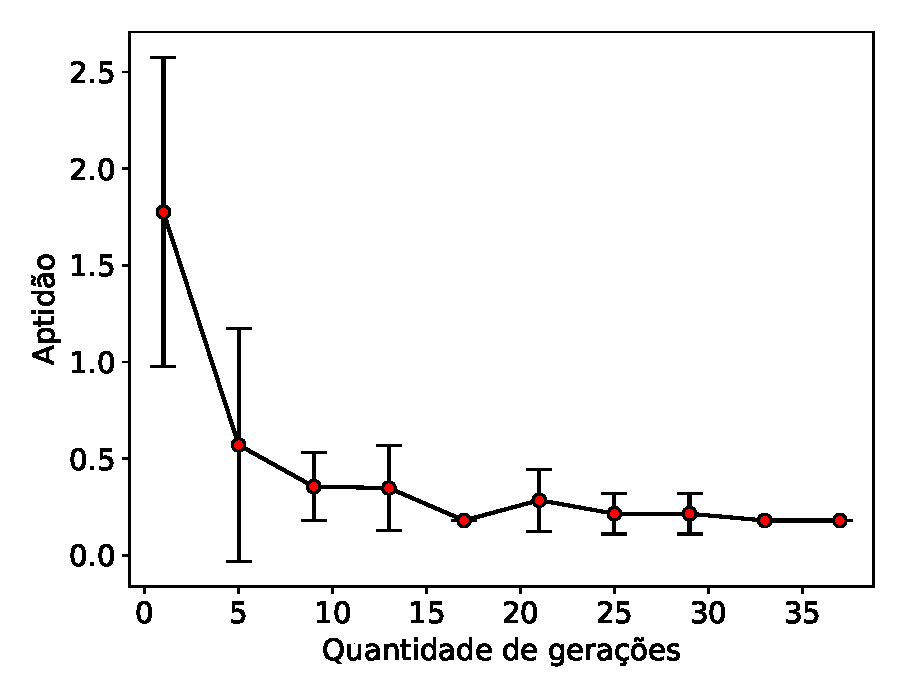
\includegraphics[scale=0.5]{../img/num_generations.eps}
		\label{fig:num_generations}
	} 
	\subfigure[]{
		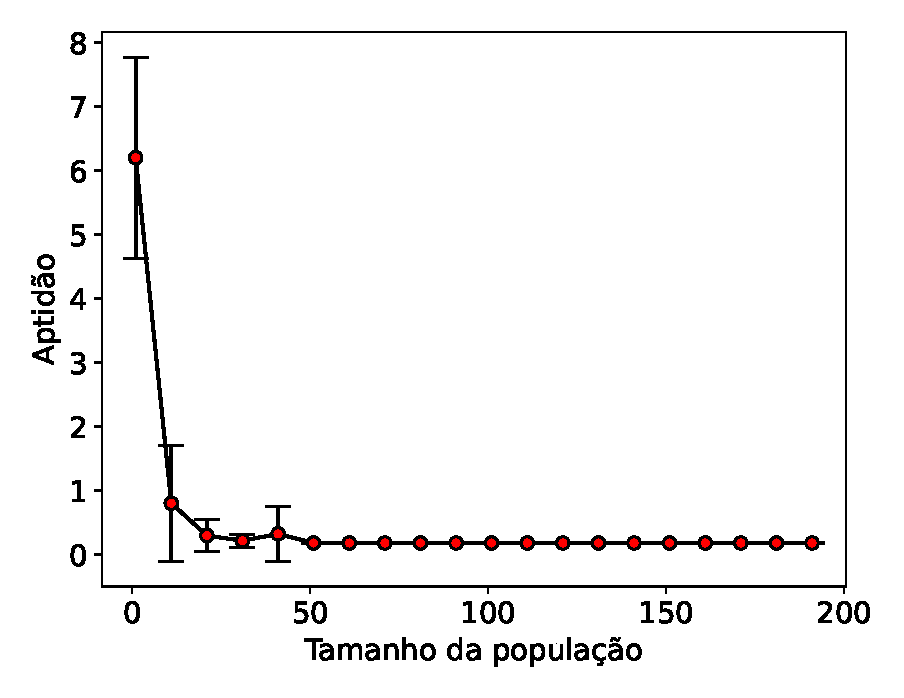
\includegraphics[scale=0.5]{../img/num_pop.eps}
		\label{fig:num_pop}
	} 
	\caption{Variação dos parâmetros.}
\end{figure}

Já na figura \ref{fig:num_bits} o número de bits é variado e quanto maior o número de bits mais números existem no espaço de busca com isso, assim como o valor ótimo pode ser obtido com mais precisão também é mais custoso achar o ponto ótimo.

Pela figura \ref{fig:num_genes} é possível observar que quanto mais genes mais o algoritmo se afastou do ótimo, isso deve-se a o aumento de dificuldade na obtenção do ótimo pela quantidade de novos genes que precisam se aproximar dos números ótimos.

\begin{figure}[!htb]
	\centering
	\subfigure[]{
		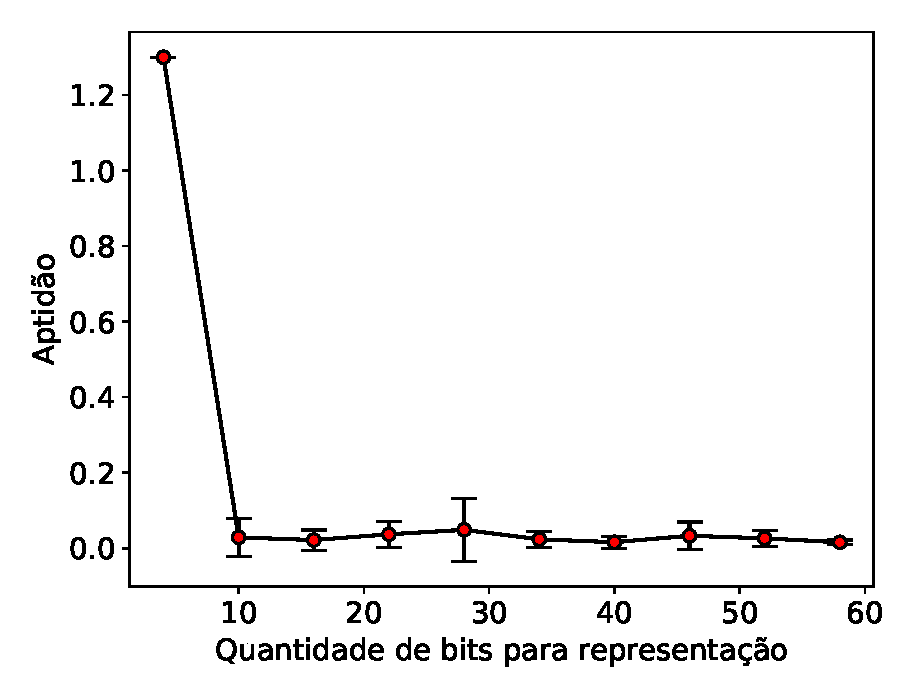
\includegraphics[scale=0.5]{../img/num_bits.eps}
		\label{fig:num_bits}
	} 
	~
	\subfigure[]{
		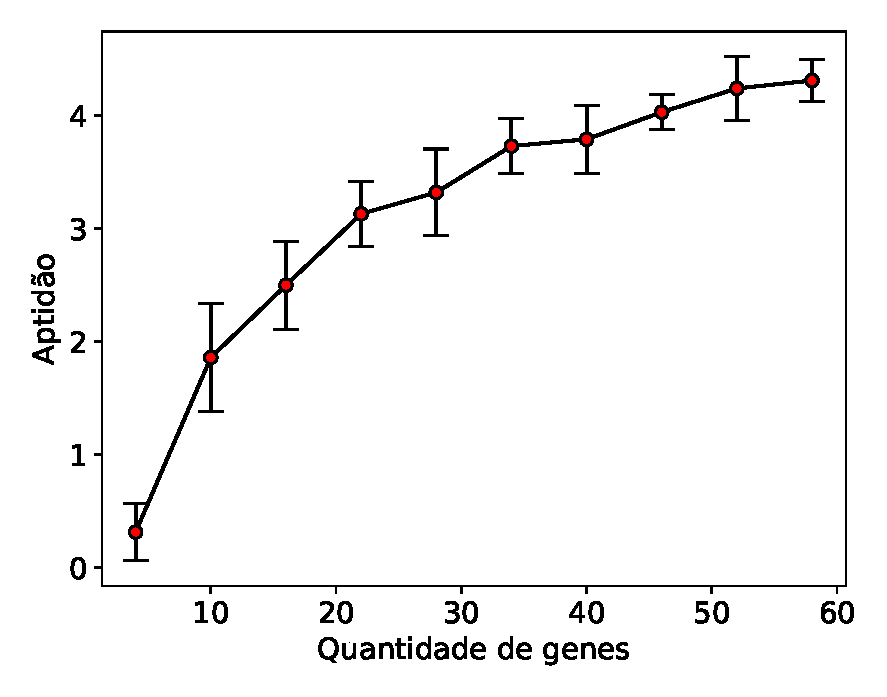
\includegraphics[scale=0.5]{../img/num_genes.eps}
		\label{fig:num_genes}
	} 
	\caption{Variação dos parâmetros}
\end{figure}
A figura \ref{fig:cross_rate} mostra que é importante ser feito cruzamento para uma busca pela solução ótima efetiva. Como o espaço de busca considerado é bem pequeno esse parâmetro e outros não apresentam um comportamento com bastante variabilidade, porém em futuros trabalhos essa análise podera ser feita de maneira mais visível.

ção precisa ter um limite se não somente ira gerar desordem na busca pelo ótimo, isso é comprovado no gráfico

No geral a figura \ref{fig:mutation_rate} mostra que a taxa de mutação so atrapalha quando a probabilidade de mutação é muito alta, pois desse modo hávera muita variação/diversificação nos valores o que causa muita desordem para ser possível fazer \emph{exploitation}.

\begin{figure}[!htb]
	\centering
	\subfigure[]{
		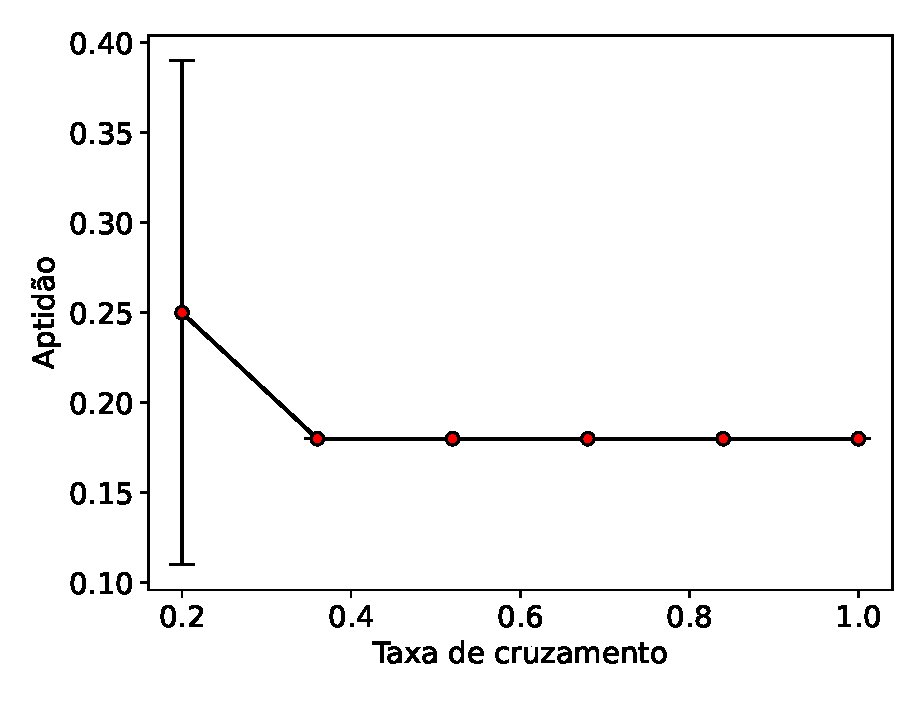
\includegraphics[scale=0.5]{../img/cross_rate.eps}
		\label{fig:cross_rate}
	} 
	~
	\subfigure[]{
		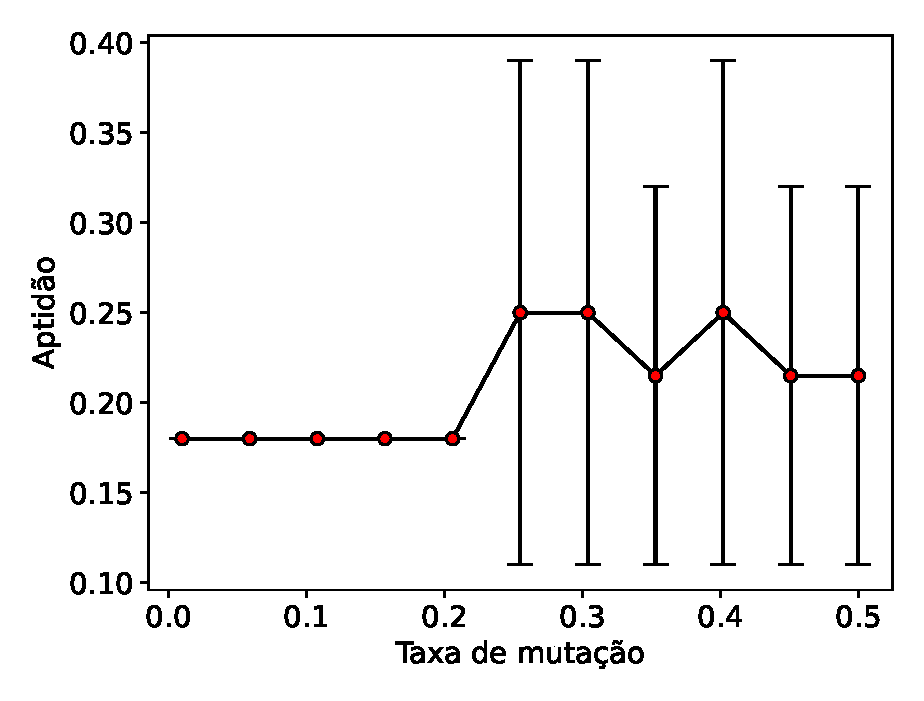
\includegraphics[scale=0.5]{../img/mutation_rate.eps}
		\label{fig:mutation_rate}
	} 

	\caption{Variação dos parâmetros}

\end{figure}

%\begin{figure}[!htb]
%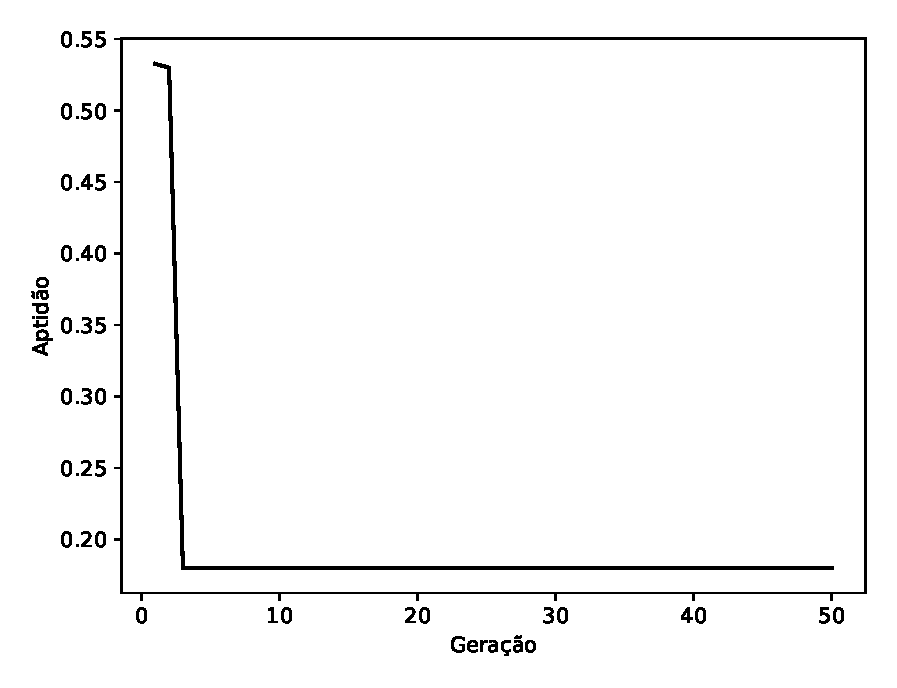
\includegraphics{../img/normal.eps}
% \caption{Execução com parâmetros padrões.}
% \label{fig:normal}
% \end{figure}

\subsection{Otimizando hiperparâmetros}
\label{sec:org5c73b33}

Agora para solucionar o problema será feito a busca pelo melhor parâmetro que soluciona o problema. Como o valor padrão para o número de bits é muito baixo, se torna muito fácil achar a solução ótima e fica sem sentido a busca pelo melhor parâmetro visto que a maioria das soluções são ótimas (ótima em relação ao domínio), devido a isso será utilizado 25 bits. Para isso será considerado os parâmetros que possuem mais impacto: gerações; população; taxa de cruzamento e taxa de mutação. A tabela \ref{tbl:hyperparameter} a seguir descreve os domínios de busca para cada parâmetro.

\begin{table}[htbp]
\caption{\label{tbl:hyperparameter}Domínio de busca de cada parâmetro.}
\centering
\begin{tabular}{ll}
\hline
\#Gerações & \{50,100\}\\
\#População & \{50,100\}\\
Taxa de cruzamento & \{0.6, 0.8, 1.0\}\\
Taxa de mutação & \{0.01, 0.05, 0.1\}\\
\hline
\end{tabular}
\end{table}

A partir da execução o \emph{top}-10 de parâmetros são descritos na tabela a seguir:

\begin{center}
\begin{tabular}{rrrrrr}
\hline
\#População & \#Gerações & Taxa de cruzamento & Taxa de mutação & Média \(F_o\) & Desvio padrão        \(F_o\)\\
\hline
100 & 100 & 0.8 & 0.01 & 3.982e-05 & 2.949474e-05\\
100 & 100 & 1.0 & 0.01 & 6.5716e-05 & 9.0926290e-05\\
100 & 100 & 0.6 & 0.01 & 0.0001981 & 0.00019136\\
50 & 100 & 0.6 & 0.01 & 0.0002714 & 0.000179354\\
50 & 100 & 0.8 & 0.01 & 0.000417 & 0.000392633\\
100 & 50 & 0.6 & 0.01 & 0.00049 & 0.000307831\\
100 & 50 & 0.8 & 0.01 & 0.0007104 & 0.000726924\\
50 & 100 & 1.0 & 0.01 & 0.00125232 & 0.00116128\\
50 & 50 & 0.8 & 0.01 & 0.0013694 & 0.001276186\\
100 & 100 & 1.0 & 0.05 & 0.0017521 & 0.002844937\\
\end{tabular}
\end{center}



É interessante se notar que os três melhores conjunto de parâmetros so se diferenciam pela taxa de cruzamento. E mesmo somente pela taxa de cruzamento é possível observar uma diferença significativa entre o \emph{top}-1 e o \emph{top}-3, assim mostrando a importancia desse parâmetro. É possível ver que as melhores soluções para esse problema não utilizam diversificação de maneira ingenua, sendo mais conservador nas operações de mutação e cruzamento. Também é importante notar que o alto valor de população e gerações é importante para essa configuração mais conservadora pois ele converge para a melhor solução lentamente.

Na figura \ref{fig:best_executions} há as execuções do algoritmo com o melhor parâmetro, é possível ver que ele chega em um valor baixo rapidamente porém continua convergindo até a solução durante as gerações. Também houve pouca variação nas execuções, como também foi mostrado na tabela, porém no começo poucas execuções demoram a descer para próximo do valor ótimo.

\begin{figure}[!htb]
	\centering
	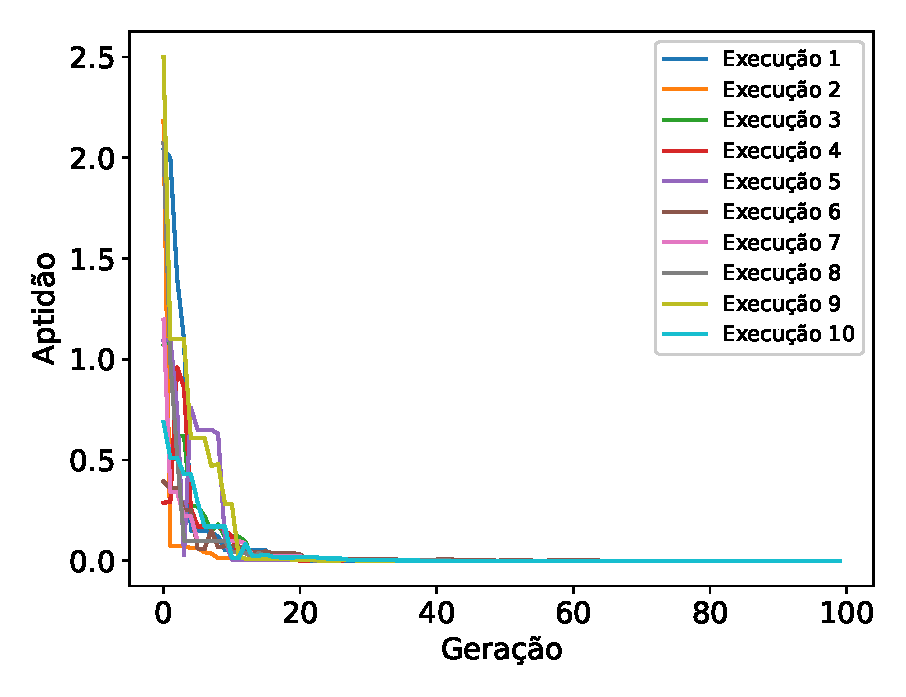
\includegraphics[scale=0.5]{../img/best_executions.eps}
	\label{fig:best_executions}
	\caption{Execuções do melhor parâmetro}
\end{figure}


\section{Conclusão}
\label{sec:orga91e6e6}

Com esse trabalho foi possível fazer a análise detalhada do comportamento de um modelo de algoritmo genético. Atráves de multiplos gráficos os parâmetros do modelo foram análisados. Como o problema a ser tratado é bem simples o algoritmo majoritariamente consegue achar o ponto ótimo do domínio.

\bibliography{doc}
\bibliographystyle{plain}
\end{document}